\documentclass[12pt]{article}
\usepackage{verbatim}
\usepackage{amsfonts}
\usepackage{graphics}
\usepackage{amsmath}
\usepackage{times}
\usepackage{appendix}
\usepackage{color}
\usepackage{multirow}
\usepackage{multicol}
\usepackage{enumerate}
\usepackage{dirtytalk}
\usepackage{fancyhdr,latexsym,amsmath,amsfonts,amssymb,amsbsy,amsthm,url}
\usepackage[margin=0.5in,footskip=0.25in]{geometry}
\usepackage{graphics,graphicx,epsfig}
\usepackage{breqn}
\usepackage{caption,subcaption,float,subfloat}
\newtheorem{theorem}{Theorem}[]
\newtheorem{lemma}{Lemma}[]
\newtheorem{remark}{Remark}[]
\newtheorem{definition}{Definition}[]
% For colored text
\usepackage[english]{babel}
% For schematic diagram
\usepackage[dvipsnames]{xcolor}
\usepackage{tikz}
%\usepackage[hyphens,spaces,obeyspaces]{url}
\usepackage{url}
\usepackage{hyperref}

\textheight=720pt \allowdisplaybreaks
\numberwithin{equation}{section}

\fancypagestyle{usual}{
  \lhead[\thepage]{}
  \chead[{\it \shortauthors}]{\sc \shorttitle}
  \rhead[]{\thepage}
  \lfoot[]{}
  \cfoot[]{}
  \rfoot[]{}
  \renewcommand{\headrulewidth}{0pt}
}

\makeatletter

\renewcommand{\section}{
  \@startsection
  {section}% name
  {1}% level
  {0pt}% indent
  {1.1\baselineskip}% beforeskip
  {0.2\baselineskip}% afterskip
  {\sc \centering}% style
}

\renewcommand{\subsection}{
  \@startsection
  {subsection}% name
  {1}% level
  {0pt}% indent
  {1.1\baselineskip}% beforeskip
  {0.2\baselineskip}% afterskip
  {\sc \centering}% style
}

\renewcommand{\subsubsection}{
  \@startsection
  {subsubsection}% name
  {1}% level
  {0pt}% indent
  {1.1\baselineskip}% beforeskip
  {0.2\baselineskip}% afterskip
  {\sc \centering}% style
}

\makeatother

\renewcommand{\thesection}{\arabic{section}}
\renewcommand\baselinestretch{1.0}

\begin{document}

\title{\large\sc Can robust risk minimization offer improved portfolio performance?: An empirical study of Indian market}
\normalsize

\author{\sc{Mohammed Bilal Girach} \thanks{Indian Institute of Technology Guwahati, Guwahati-781039, Assam, India, e-mail: m.girach@iitg.ac.in}
\and \sc{Shashank Oberoi} \thanks{Indian Institute of Technology Guwahati, Guwahati-781039, Assam, India, e-mail: s.oberoi@iitg.ac.in}
\and \sc{Siddhartha P. Chakrabarty} \thanks{Indian Institute of Technology Guwahati, Guwahati-781039, Assam, India, e-mail: pratim@iitg.ac.in,
Phone: +91-361-2582606, Fax: +91-361-2582649}}
\date{}
\maketitle
%\thispagestyle{empty}
\begin{abstract}

We begin with a discussion on the classical Markowitz portfolio optimization, its drawbacks and consequent motivation of the alternate approach of robust portfolio optimization. We present the extension of the robust optimization framework in the case of VaR and CVaR minimization. We perform an empirical study of VaR and CVaR vis-\`a-vis their robust counterparts, namely, Worst-Case VaR and Worst-Case CVaR, using the market data as well as simulated data. After discussing the practical usefulness of the robust optimization approaches from various standpoints, we infer various takeaways. The robust models in the case of VaR and CVaR minimization exhibit superior performance with respect to their base versions in the cases involving higher number of stocks and simulated setup respectively.

{\it Keywords: Robust portfolio optimization; CVaR; VaR; S\&P BSE 30; S\&P BSE 100}

\end{abstract}

\section{Introduction}
\label{Introduction}

Investment in an individual security always has an associated risk, which can be minimized through diversification, a process involving  investment in a portfolio consisting of several securities. For optimal allocation of weights in a diversified portfolio, one of the well-established methods is the classical mean-variance portfolio optimization introduced by Markowitz \cite{Markowitz1,Markowitz2}. Mean and covariance matrix of returns of securities are used as the measures for giving a quantitative sense to the return and the risk, respectively, of the portfolio. Despite being considered as the most basic theoretical framework in the field of portfolio optimization, there are several drawbacks associated with incorporating the Markowitz model in a practical setup.


Theoretically, Markowitz based portfolio optimization can result in assigning extreme weights to the securities comprising the portfolio. However, investment in securities can not be made in such extreme positions like large short positions if one takes active trading into account. Such kind of scenarios can be avoided by introducing appropriate constraints on the weights.  Black and Litterman \cite{Black} argued that there is an added disadvantage since there are high chances of the optimal portfolio lying in the neighborhood of the imposed constraints. Thus, imposition of constraints leads to strong dependence of the constructed portfolio upon the constraints. For example, disallowing short sales often results in assigning zero weights to many securities and largely positive weights to the securities having small market capitalization. 

One of the most major limitations of the mean-variance model is the sensitivity of the optimal portfolios to the errors in the estimation of return and risk parameters. These parameters are estimated using sample mean and sample covariance matrix, which are maximum likelihood estimates (MLEs) (calculated using historical data) under the assumption that the asset returns are normally distributed. According to DeMiguel and Nogales \cite{demiguel}, since the efficiency of MLEs is extremely sensitive to deviations of the distribution of asset returns from the assumed normal distribution, it results in the optimal portfolios being vulnerable to the errors in estimation of input parameters. Additionally, the historical data neglects various other market factors and is not an accurate representation for estimates of future returns. Taking into account the above reasons, Michaud \cite{Michaud} argued that the mean-variance analysis tends to maximize the impact of estimation errors associated with the return and the risk parameters for the securities. As a result, Markowitz portfolio optimization often overweighs (underweighs) the securities having higher (lower) expected return, lower (higher) variance of returns and negative (positive) correlation between their returns. Labelling the model as \say{estimation-error maximizers}, he stated that it often leads to financially counter-intuitive portfolios, which, in some cases, perform worse than the equal-weighted portfolio. Broadie \cite{Broadie} investigated the error maximization property of mean-variance analysis. Accordingly, he conducted a simulation based study to compare the estimated efficient frontier with the actual frontier computed using true parameter values. He observed that points on the estimated efficient frontier show superior performance as compared to the corresponding points on the actual frontier. He supported his argument of over-estimation of expected returns of optimal portfolios through his simulated results of obtaining the estimated frontier lying above the actual frontier. Additionally, he pointed out that non-stationarity in the data of returns can further increase the errors in computing the efficient frontier. Chopra and Ziemba \cite{Chopra} performed the sensitivity analysis of performance of optimal portfolios by studying the relative effect of estimation errors in means, variances and covariances of security returns, taking the investors' risk tolerance into consideration as well. They observed that at a high risk tolerance (to be defined in later chapters) of around fifty, cash equivalent loss for estimation errors in means is about eleven times greater than that for errors in variances or covariances. Accordingly, they pointed out that if the investors have superior estimates for means of security returns, they should prefer using them over the sample means calculated from historical data. Best and Grauer \cite{Best1,Best2} also arrived at similar conclusions by studying the sensitivity of weights of optimal portfolios with respect to changes in estimated means of returns on individual securities. Further, on imposition of no short selling constraint on the securities, they observed that a small change in estimated mean return of an individual security can assign zero weights to almost half the securities comprising the portfolio, which is counter-intuitive.

The discussed literature arrives at a common conclusion that the optimal portfolios are extremely sensitive towards the estimated values of input parameters, particularly expected returns of individual securities. In order to address this issue, there has been significant progress in recent years in the area of robust portfolio optimization. Several methods have been proposed in this area. \textbf{We are particularly interested in the class of methods that enhance robustness by optimizing the portfolio performance in worst-case scenarios.} 

Significant efforts have been made towards formulating these kinds of approaches from Markowitz based mean-variance analysis. The robust optimization approach incorporates uncertainty in the input parameters directly into the optimization problem. T{\"u}t{\"u}nc{\"u} and Koenig \cite{tutuncu} described uncertainty, using an uncertainty set that includes almost all possible realizations of the uncertain input parameters. Accordingly, they formulated the problem of robust portfolio optimization by optimizing the portfolio performance under the worst possible realizations of the uncertain input parameters. They conducted numerous experiments applying the robust allocation methods to the market data and concluded that robust optimization can be considered as a viable asset allocation alternative for conservative investors.
According to Ceria and Stubbs \cite{Ceria}, the standard approach of robust optimization is too conservative. They argued that it is too pessimistic to adjust
the return estimate of each asset downwards. Accordingly, they introduced new variants of robust optimization, taking into account the estimation errors in input parameters while formulating the optimization problem. They observed that the constructed robust portfolios perform superior in comparison to those constructed using mean-variance analysis in most of the cases but not in each month with certainty. Utilizing the standard framework of robust optimization, Scherer \cite{Scherer} showed that robust methods are equivalent to Bayesian shrinkage estimators and do not lead to significant change in the efficient set. Constructing an example, he showed that robust portfolio does not outperform out of the sample in comparison to the Markowitz portfolio, especially in the case of low risk aversion and high uncertainty aversion. He also argued that performance of robust portfolio is dependent upon the consistency between uncertainty aversion and risk aversion which is quite complicated. Santos \cite{santos} performed similar experiments to compare two types of robust approaches, namely, the standard robust optimization discussed in Scherer's work \cite{Scherer} and zero net alpha-adjusted robust optimization proposed by Ceria and Stubbs \cite{Ceria}, with the traditional optimization methods. The empirical results indicated better performance of robust approaches in comparison to the portfolios constructed using mean-variance analysis in the case of simulated data unlike in the case of real market data. 

There are several limitations of the mean-variance framework such as sensitivity to errors in data as well as in the estimation of mean and variance of the underlying distribution. Furthermore, another criticism usually associated with the mean-variance setup is the use of standard deviation as a measure of risk. On the other hand, from a practitioners' point of view, the upside and downside risk cannot be perceived in the same way, because most of the times, the upside risk can improve the overall performance of the portfolio whereas the downside fluctuation usually brings impactful losses. Variance is not a reliable or appropriate  risk measure, if the underlying distribution is leptokurtic. In order to address these issues, models involving other measures of risk have been developed and accordingly their corresponding robust models have been studied as well. In the forthcoming chapters, we will elaborately discuss some of the most widely measures of risk like Value at Risk (VaR) and Conditional Value at Risk (CVaR) and also study their corresponding robust worst case formulations.

Unlike the mean-variance setup, VaR framework takes into account the probability of losses \cite{var96}. Ghaoui et al. \cite{ghaoui03} defined VaR, at confidence level $1-\epsilon$, as the minimum value of $\gamma$ such that the probability of loss exceeding $\gamma$ is less than $\epsilon$. Though VaR takes probability of losses into account, it has its own limitations. For the computation part, it requires the knowledge of the whole distribution. The computation also involves high dimensional numerical integration which may not be tractable at times and also there hasn't been an extensive research on methods using Monte Carlo simulations \cite{var96} for the design of the portfolio. Black and Litterman \cite{Black}, Pearson and Ju \cite{ju98} discussed the issues regarding the computational difference between the true VaR and the calculated VaR and determined that the error in the computation of the VaR can be attributed to errors in the estimation of the first and second moments of the asset returns.

The concept of worst-case VaR not only allows for approaching the solution in a more tractable way, but also relaxes the assumptions on the information known to us apriori. Here, we assume that only partial information about the underlying distribution is known. We also assume that the distribution of the asset returns belong to a family of allowable probability distributions $\mathcal{P}$ \cite{ghaoui03}. For example, given component wise bounds of ($\hat{\boldsymbol{\mu}}$,  $\Sigma$), $\mathcal{P}$ could comprise of normally distributed random variables with $\hat{\boldsymbol{\mu}}$ and $\Sigma$ as the moments' pairs.


Despite its popularity as a measure of downside risk, VaR has received a fair amount of criticism \cite{capinski_risk,zhu,lim}. VaR for a diversified portfolio may exceed that for an investment in a single asset. Thus, one of the major limitations of VaR is the lack of sub-additivity in the case of general distributions. In accordance with this observation, VaR is not a coherent measure of risk as per the definition laid out by Artzner et al \cite{artzner}. Secondly, VaR does not provide any information on the size of losses in adverse scenarios \textit{i.e,} those beyond the confidence level ($1-\epsilon$). Additionally, VaR is non-convex and non-differentiable when incorporated into portfolio optimization problem. As a result, it becomes difficult to optimize VaR since global minimum may not exist. 

Conditional Value-at-Risk (CVaR), introduced by Rockafellar and Uryasev \cite{rockafellar1,rockafellar2}, has addressed various concerns centred around VaR. For continuous distributions, CVaR is the expected loss conditioned on the loss outcomes exceeding VaR. In recent years, CVaR has emerged as a viable risk measure in portfolio optimization problems over its use in reducing downside risk. It has been proved by Pflug \cite{pflug} and Acerbi and Tasche \cite{acerbi} that CVaR is a coherent measure of risk. Accordingly, it follows the property of sub-additivity. Therefore, CVaR can be minimized through investment in a diversified portfolio. Unlike VaR, CVaR takes into consideration the impact of losses beyond the confidence level ($1-\epsilon$) \cite{capinski_risk}. Also, the minimization of CVaR is a convex optimization problem \cite{lim}.

Similar to Markowitz optimization and VaR minimization, there is an issue of lack of robustness in the classical framework of CVaR minimization. Computing CVaR requires the complete knowledge of the return distribution as argued by Zhu and Fukushima \cite{zhu}. They have addressed this shortcoming of the classical CVaR (henceforth, referred to as base-case CVaR) by proposing a new risk measure, namely, Worst-Case CVaR (WCVaR). 

The rest of the paper is organized as follows. In section \ref{Risk_Minimization_Approaches}, we discuss the tractable formulations of the downside risk minimization methods used in the work. Section \ref{Computational_Results} presents the empirical results observed on comparison of the performance of robust risk minimization models with their classical counterparts. Section \ref{Discussion} focuses on analyzing the practical viability of the robust models from the standpoint of number of stocks, sample size and type of data. In section \ref{Conclusion}, we sum up the key inferences from this work .

\section{Risk Minimization Approaches}
\label{Risk_Minimization_Approaches}
In this section, we discuss the mathematical formulations of the problems of optimizing VaR and CVaR along with their robust counterparts, namely, WVaR and WCVaR respectively.
\subsection{Value at Risk (VaR)}
Mathematically, the VaR is defined as,
\begin{equation}
\begin{split}
V(\mathbf{x}) = \min \, \left\{ \gamma :  \, P\left\{\gamma \leq -r(\mathbf{x},\boldsymbol{\mu})\right\} \leq \epsilon \right\},  \\
\end{split}
\label{fig:var_basic}
\end{equation}
where $\epsilon \in (0,1)$. When we deal with mean-variance setup, only the mean and the variance \textit{i.e., the first and the second moments} of the asset returns are required, but in the VaR framework, the knowledge of the entire distribution is necessary for the computation part. If the underlying distribution is Gaussian with the moments' pair as ($\hat{\boldsymbol{\mu}}$, $\Sigma$), then VaR can be computed via the following analytical form:
\begin{equation}
\begin{split}
V(\mathbf{x}) = \kappa(\epsilon)\sqrt{\mathbf{x}^{\top}\Sigma \mathbf{x}} - \hat{\boldsymbol{\mu}}^{\top}\mathbf{x},
\end{split}
\label{eqn:kappa_eqn}
\end{equation}
where $\kappa(\epsilon) = -\Phi^{-1}(\epsilon)$ with $\Phi(z)$ representing the cumulative distribution for standard normal random variable. In practice, the value of the $\kappa(\epsilon)$ can be determined only if the cumulative distribution function of the underlying distribution is known apriori. However, if the distribution is unknown, then we have to rely on the Chebyshev's inequality. The bound (upper) obtained due to Chebyshev's only requires the knowledge of the first two moments' pair. We call a bound to be exact if the upper bound is attained. If not, we use the bound given by Bertsimas and Popescu \cite{bert05} \textit{i.e.,} $\displaystyle{ \kappa(\epsilon) = \sqrt{\frac{1-\epsilon}{\epsilon}}}$. Finally, we formulate the generalised VaR as follows:
\begin{equation}
\begin{split}
\min \, \kappa(\epsilon)\sqrt{\mathbf{x}^{\top}\Sigma \mathbf{x}} - \hat{\boldsymbol{\mu}}^{\top}\mathbf{x} \quad \text{subject to } \quad \mathbf{x} \in \mathcal{X},
\end{split}
\label{fig:var_general}
\end{equation}
where $\kappa(\epsilon)$ is an appropriate factor of risk chosen in accordance with the underlying distribution of asset returns and $\mathcal{X} = \left\{ \mathbf{x} : \mathbf{x}^{\top}\mathbf{1} = 1 \text{ and } \mathbf{x} \geq 0 \right\}$. The function $V(\mathbf{x})$ is convex and the global optimum can be obtained using techniques like interior-point methods and second order cone programming (SOCP).

\subsection{Worst-Case VaR}
Given a probability (confidence) level $\epsilon$, the worst-case VaR can be formulated as 
\begin{equation}
\begin{split}
V_{\mathcal{P}}(\mathbf{x}) = \min \, \left\{\gamma : \, \sup_{P \in \mathcal{P}} P\left\{\gamma \leq -r(\mathbf{x},\boldsymbol{\mu})\right\} \leq \epsilon \right\},
\end{split}
\label{fig:wc_var_basic}
\end{equation}
where $\mathcal{P}$ is the family of allowable probability distributions. Accordingly, the robust formulation can be written as 
\begin{equation}
\begin{split}
V_{\mathcal{P}}^{\text{opt}}(\mathbf{x}) = \min \, V_{\mathcal{P}}(\mathbf{x}) \quad \text{subject to} \quad \mathbf{x} \in \mathcal{X}, 
\end{split}
\label{fig:wc_var_general}
\end{equation}

The above optimization problems can be computed by a semi-definite programming (SDP) problem which again uses the above mentioned interior-point methods. We deal with the high dimensional problems by using bundle methods which are mainly used for large-scale (sparse) problems.

Motivated by the work of separable uncertainty sets by T{\"u}t{\"u}nc{\"u} and Koenig \cite{tutuncu}, one can view the robust formulation given by Ghaoui et al. \cite{ghaoui03} in case of Polytopic uncertainty, as a robust formulation of WVaR involving separable uncertainty (section: \ref{ssec:sep}). Accordingly, the formulation of the optimization problem for worst case VaR is,
\begin{equation}
\begin{split}
\min \, \kappa(\epsilon)\sqrt{\mathbf{x}^{\top}\overline{\Sigma}\mathbf{x}} - \underline{\hat{\boldsymbol{\mu}}}^{\top}\mathbf{x} \quad \text{subject to } \quad \mathbf{x} \in \mathcal{X},
\end{split}
\label{fig:var_poly}
\end{equation}
where $\overline{\Sigma}$ and $\underline{\hat{\boldsymbol{\mu}}}$ are higher bound for covariance matrix and lower bound for the estimated mean of asset returns respectively. We obtain these values by using the Non-Parametric Bootstrap algorithm where the type of distribution is unknown. This can also be viewed as a robust formulation involving polytopic uncertainty because \say{Separable uncertainty} is a special case of \say{Polytopic uncertainty}. In case of models involving ellipsoidal uncertainty sets, the robust worst-case VaR formulation is not that trivial and such models mainly revolve around the assumption of factor models.

\subsection {Conditional Value at Risk (CVaR)}
For $\epsilon \in (0,1)$ , CVaR, at confidence level $1-\epsilon$, is defined as:
\begin{equation}
\label{eq:6.1}
CVaR_{\epsilon}(\mathbf{x}) \triangleq \frac{1}{\epsilon} \, \int \limits_{-\mathbf{r}^{\top}\mathbf{x} \geq VaR_{\epsilon}(\mathbf{x})} p(\mathbf{r})  d\mathbf{r}
\end{equation}
where $\mathbf{r}$ is the random return vector having probability density function $p(\mathbf{r})$ and $\mathbf{x}$ is the weight vector for a portfolio.

As proved by Rockafeller and Uryasev \cite{rockafellar1} , $CVaR_{\epsilon}(\mathbf{x})$, defined in equation (\ref{eq:6.1}), can be transformed into: 
\begin{equation}
\label{eq:6.4}
CVaR_{\epsilon}(\mathbf{x}) = \min_{\gamma \in \mathcal{R}^{n}} F_{\epsilon}(\mathbf{x},\gamma)
\end{equation}
where $n$ is number of assets in the portfolio and $F_{\epsilon}(\mathbf{x},\gamma)$ is defined as:
\begin{equation}
\label{eq:6.5}
 F_{\epsilon}(\mathbf{x},\gamma) \triangleq \gamma \, + \, \frac{1}{\epsilon} \, \int \limits_{\mathbf{r} \in \mathcal{R}^{n}} [-\mathbf{r}^{\top}\mathbf{x}-\gamma]^{+} p(\mathbf{r})  d\mathbf{r}
\end{equation}
In the above equation, $[t]^{+}=\max \{t,0\}$. The problem of approximation of the integral involved in the equation (\ref{eq:6.5}) can be dealt by sampling the probability distribution of $\mathbf{r}$ as per its density $p(\mathbf{r})$. Assuming there are S samples, $\{ \mathbf{r}_{1}, \mathbf{r}_{2}, .., \mathbf{r}_{i},..,\mathbf{r}_{S}\}$ for the return vector $\mathbf{r}$, $ F_{\epsilon}(\mathbf{x},\gamma)$ can be approximated as \cite{rockafellar1}:
\begin{equation}
\label{eq:6.6}
 F_{\epsilon}(\mathbf{x},\gamma) \approx \gamma \, + \, \frac{1}{S \, \epsilon} \, \sum_{i=1}^{S} [-\mathbf{r}_{i}^{\top}\mathbf{x}-\gamma]^{+} 
\end{equation}
In accordance with above approximation, the problem of minimization of classical CVaR, assuming no short-selling constraints, can be formulated as the following Linear Programming Problem (LLP) \cite{rockafellar1,zhu}:
\begin{equation}
\label{eq:6.7}
\begin{split}
& \min_{(\mathbf{x},\mathbf{u},\gamma,\theta)} \, \theta \, \, s.t. \\
& \mathbf{x}^{\top}\mathbf{1}=1, \mathbf{x} \geq \mathbf{0}, \\
& \gamma \, + \, \frac{1}{S \, \epsilon} \mathbf{1}^{\top}\mathbf{u} \leq \theta, \\
& u_{i} \geq -\mathbf{r}_{i}^{\top}\mathbf{x}-\gamma, \, u_{i} \geq 0, \, i=1,2,..,S. \\
\end{split}
\end{equation}
where the auxiliary vector $\mathbf{u} \in \mathcal{R}^S$ and $\theta$ is the auxiliary variable that is optimized to obtain the optimal value of the Base-Case CVaR.

\subsection {Worst-Case CVaR}
For a fixed weight vector $\mathbf{x}$, at confidence level $1-\epsilon$, WCVaR is defined as:
\begin{equation}
\label{eq:6.2}
WCVaR_{\epsilon}(\mathbf{x}) \triangleq \sup_{p(\mathbf{r}) \in \mathcal{P}}CVaR_{\epsilon}(\mathbf{x})
\end{equation}
where we assume that the density function $p(\mathbf{r})$ of returns belongs to a set $\mathcal{P}$ of probability distributions. Zhu and Fukushima \cite{zhu} have proved the coherence of WCVaR as a risk measure by analyzing it in terms of worst-case risk measure $\rho_{w}$:
\begin{equation}
\label{eq:6.3}
\rho_{w}(X) \triangleq \sup_{p(\mathbf{r}) \in \mathcal{P}} \rho (X)
\end{equation}

We skip discussion on WCVaR formulations using box uncertainty set and ellipsoidal uncertainty set since they require a set of possible return distributions to be assumed so as to obtain bounds and scaling matrix respectively. However, our problem setup doesn't involve a set of return distributions since we make use of only market data (where return distribution is not known) and simulated data (where we generate a known return distribution).

We describe the formulation of the optimization problem involving WCVaR by assuming that the return distribution belongs to a set of distributions comprising of all possible mixtures of some prior likelihood distributions \cite{zhu}. Mathematically, it is assumed that:
\begin{equation}
\label{eq:6.8}
p(\mathbf{r}) \in \mathcal{P}_{M} \triangleq \bigg\{ \sum_{j=1}^{l} \lambda_{j}p^{j}(\mathbf{r}) \, : \, \sum_{j=1}^{l}\lambda_{j}=1, \lambda_{j} \geq 0,j=1,2,..,l \bigg\}
\end{equation}
In the above equation, $p^{j}(\mathbf{r})$ denotes the $j^{th}$ likelihood distribution and $l$ is the number of the likelihood distributions. In accordance with above assumption of mixture distribution uncertainty (that involves $\mathcal{P}_{M}$ as a compact convex set) , $WCVaR_{\epsilon}(\mathbf{x})$, defined in equation (\ref{eq:6.2}), can be rewritten as the following min-max problem \cite{zhu}: 
\begin{equation}
\label{eq:6.9}
\begin{split}
& WCVaR_{\epsilon}(\mathbf{x}) = \min_{\alpha \in \mathcal{R}} \max_{j \in \mathcal{L} } F_{\epsilon}^{j}(\mathbf{x},\gamma) \, , \, \text{where} \\
& \mathcal{L} \triangleq \{ 1,2,..,l \} \\
& F_{\epsilon}^{j}(\mathbf{x},\gamma) \triangleq \gamma \, + \, \frac{1}{\epsilon} \, \int \limits_{\mathbf{r} \in \mathcal{R}^{n}} [-\mathbf{r}^{\top}\mathbf{x}-\gamma]^{+} p^{j}(\mathbf{r})  d\mathbf{r} \\
\end{split}
\end{equation}
Similar to the case involving classical CVaR in previous subsection, $F_{\epsilon}^{j}(\mathbf{x},\gamma)$ can be approximated via discrete sampling as:
\begin{equation}
\label{eq:6.10}
F_{\epsilon}^{j}(\mathbf{x},\gamma) \approx \gamma \, + \, \frac{1}{S_{j} \, \epsilon} \, \sum_{i=1}^{S_{j}} [-\mathbf{r}_{i,j}^{\top}\mathbf{x}-\gamma]^{+}
\end{equation}
In the above equation, $\mathbf{r}_{i,j}$ is the $i^{th}$ sample of the return with respect to $j^{th}$ likelihood distribution and $S_{j}$ is the number of samples corresponding to $j^{th}$ likelihood distribution. Accordingly, assuming non-negative weights, the problem of minimization of WCVaR over a feasible set of portfolios can be formulated as the following LLP \cite{zhu}:
\begin{equation}
\label{eq:6.11}
\begin{split}
& \min_{(\mathbf{x},\mathbf{u},\gamma,\theta)} \, \theta \, \, s.t. \\
& \mathbf{x}^{\top}\mathbf{1}=1, \mathbf{x} \geq \mathbf{0}, \\
& \gamma \, + \, \frac{1}{S_{j} \, \epsilon} \mathbf{1}^{\top}\mathbf{u}^{j} \leq \theta, \, \, j=1,2,..,l,\\
& u_{i}^{j} \geq -\mathbf{r}_{i,j}^{\top}\mathbf{x}-\gamma, \, u_{i}^{j} \geq 0, \, \, i=1,2,..,S_{j}, \, \, j=1,2,..,l. \\
\end{split}
\end{equation}
In the above equation, the auxiliary vector $\mathbf{u}=(\mathbf{u}^{1} ; \mathbf{u}^{2} ; .. ; \mathbf{u}^{l}) \in \mathcal{R}^{S}$ where $\displaystyle{S=\sum_{j=1}^{l}S_{j}}$ and $\theta$ is the auxiliary variable whose optimization yields the optimal value of the Worst-Case CVaR..

\section{Computational Results}
\label{Computational_Results}

\subsection{VaR vis-\`a-vis WVaR}

We carry out the comparative analysis on the performance of the optimal portfolios obtained when VaR (referred as \say{Base VaR} from hereon) and WVaR are incorporated as measures of risk in the robust portfolio optimization problem. We use the Sharpe Ratio (SR) as a metric to compare the performance of the portfolios. Since the yield for Treasury Bill in India from 2016 to 2018 has been found to oscillating around $6\%$ \cite{rbi}, so, we have assumed the annualized risk-free rate to be equal to $6\%$.

We perform the empirical analysis for the available historical data for S\&P BSE 30 $(N = 31)$ and S\&P BSE 100 $(N = 98)$. For the first scenario $(N = 31)$ , we use the daily log-returns based on daily adjusted close price of the 31 stocks comprising BSE 30 (data source: Yahoo Finance \cite{yf}). Accordingly, we have considered the period from December 18, 2017 to September 30, 2018 (both inclusive) comprising of a total of 194 active trading days. For the second scenario $(N = 98)$, we use the log-returns based on daily adjusted close price data of the 98 stocks comprising S\&P BSE 100 (data source: Yahoo Finance \cite{yf}) with the period spanning from December 18, 2016 to September 30, 2018. The reason behind this setup is to observe the trends/patterns in the performance of the portfolio when the number of stocks taken into consideration for constructing the optimal portfolio are changed. Furthermore, we also analyze the performance of the portfolio when in place of real market data, simulated data with true moments' pair is fed to the robust optimization problem. We dive one step further deep in above setup and vary the number of simulations to observe the changes in the performance of the optimal portfolio with increasing the number of simulations. For the above cause, we simulate two data-sets with true moments' pair, one with exact number of samples as in the available real market data, say, $\zeta \, (\leq 1000)$ and another with a large number of samples, say 1000. We also use the same setup in order to analyze the performance of the portfolio when different type of data is taken into consideration \textit{i.e.,} real market and simulated data. For the computational part of the robust formulation, we choose $\mathcal{P}$ to be family of distribution with the first and the second moments as the true mean and variance of the historical data. As the knowledge of the distribution is unknown, we use $\kappa$ from equation (\ref{eqn:kappa_eqn}), where we only consider the values of $\epsilon$ to be in (0,0.1) \textit{i.e.,} the confidence level is greater than or equal to 90\% In the following subsections, we analyze each scenario in detail with appropriate figures and tables. We allow a slight notational abuse and refer the model which uses Base VaR/ WVaR as a measure of risk as VaR and WVaR respectively. We start our discussion with smaller number of stocks for which we obtain data from S\&P BSE 30 and accordingly compute the log returns from the asset values.

\subsubsection{Performance with $N=31$ Assets}
We proceed with the analysis of the performance of the portfolio when real market data is used to construct the optimal portfolio. From Figure \ref{fig:5.1} one can observe that the performance of the portfolio is better when basic definition of VaR is used in the optimization problem. The Base VaR model outperforms the WVaR model over the complete range of $\epsilon$. For a better understanding of the trends, we mainly tabulated the values of Sharpe ratio for the optimal portfolios obtained with different values of $\epsilon$ in Table \ref{tab:5.1}. We can observe that the average value of Sharpe ratio is more for Base VaR model when compared to WVaR model and is obvious from the Figure \ref{fig:5.1}.

Now, we move to the domain of the simulated data. Firstly, we discuss the trends in the performance of the optimal portfolio when the number of the samples ($\zeta$) generated are same as there are in the real market data. We observe from the Figure \ref{fig:5.2} that there is hardly any difference in trends of the performance when we used $\zeta$ number of simulations when compared to the real market data. Also from Table \ref{tab:5.2}, we can observe that the Base VaR model exhibits superior performance over WVaR model on the complete range of $\epsilon$.

Since the model with $\zeta$ number of samples, results in the same trends as in the real market data, we now consider the case where we simulated larger number of samples, say 1000 with a justification, that larger the number of samples, less is the difference between true moments' pair with their computed counterparts. In this case, from Figure \ref{fig:5.3}, we observe that the WVaR model delivers better performance than the Base VaR model in the $\epsilon$ interval of (0, 0.04]. So, for more conservative investors, WVaR model will benefit more than the corresponding VaR model. In the Table \ref{tab:5.3}, one can cross-check the observation made above, the WVaR model performs better than Base VaR model in the interval (0, 0.04] of $\epsilon$. However, the average values remains almost equal because after the interval (0, 0.04], the Base VaR model outperforms the WVaR model. So, we conclude that in this case, both Base VaR and WVaR models are indifferent from the perspective of a rational investor.

We now extend the same type of analysis for a larger set of stocks for which we obtain data from S\&P BSE 100 ($N = 98$).

\subsubsection{Performance with $N=98$ Assets}
In the same lines, we begin our discussion of analyzing the performance of the Base VaR and WVaR models when real market data from S\&P BSE 100 is taken into consideration. We present the empirical results in Figure \ref{fig:5.4} and tabulate the observations in Table \ref{tab:5.4}. One can observe from the plot that the WVaR model exhibits superior performance in comparison to the corresponding Base VaR model on the entire range of $\epsilon$. This observation can also be quantitatively justified by Table \ref{tab:5.4} where the Sharpe Ratios of the portfolios obtained from WVaR model is greater than that of Base VaR model.

The same type of trend is observed for $N=98$ stocks in the case of simulated data as well, when the number of simulations equals $\zeta$ \textit{i.e.,} the number of instances available in the real market data of S\&P BSE 100. From Figure \ref{fig:5.5} and the Table \ref{tab:5.5}, we infer that the WVaR model performs better than the Base VaR model when Sharpe ratio is used as performance measure for every $\epsilon \in$ (0,0.1).

Lastly, we consider the case where we simulated larger number of samples in order to distinguish the fluctuations in the performance of the portfolio when number of simulations are varied. Similar kind of inferences can be drawn from Figure \ref{fig:5.6} and Table \ref{tab:5.6}. The optimal portfolios obtained from the WVaR model have greater values of Sharpe ratio when compared to those obtained from Base VaR model irrespective of the value of $\epsilon$.

\subsection{CVaR vis-\`a-vis WCVaR}

Similar to the computational analysis of robust methods in VaR minimization, we perform empirical analysis of the Worst-Case CVaR  model vis-\`a-vis the Base-Case CVaR model, making use of the historical market data and simulated data. Taking into consideration the number of stocks $N$, the comparative study is conducted under two scenarios, namely, $N=31$ and $N=98$. These numbers represent the number of stocks in S\&P BSE 30 and S\&P BSE 100 indices, respectively.

For each scenario, we use the same three sets of data as used in the performance analysis of robust approaches in Chapters 3 and 5 \textit{i.e,} a set of historical market data comprising daily log-returns and two sets of simulated data. The first set of simulated data comprises of the number of sample returns matching the number of return instances of the historical market data, say $\zeta (<1000)$. On the other hand, the second set has a larger number of samples, namely, 1000.

During computation of the Base-Case CVaR model, $S$ in equation (\ref{eq:6.7}) is set equal to the number of return samples, \textit{i.e,} either $\zeta$ or $1000$, depending upon the set of data used. We perform computation of the Worst-Case CVaR model, as formulated in equation (\ref{eq:6.11}), for values of $l$ in $\{2,3,4,5\}$ by setting $\displaystyle{S_{j}=\frac{S}{l}}$ where $\displaystyle{j \in \{1,2,..,l \}}$. Note that $l=1$ yields the same case as the classical CVaR model. We do not include larger values of $l$ in the discussion on the empirical results since this leads to a great decrease in the sample size for the likelihood distributions.

We perform comparative analysis of the Worst-Case CVaR model with respect to the Base-Case CVaR model using the Sharpe Ratio of the constructed portfolios having confidence level greater than $90\%$, \textit{i.e,} $\epsilon \in (0,0.1)$. Similar to preceding chapters, for computing the Sharpe Ratio, we assume the annualized risk free rate equal to $6\%$. In the following subsections, we present the computational results for the two scenarios.

\subsubsection{Performance with $N=31$ Assets}

We begin with the analysis for $N=31$ assets, in the case of the historical market data having log-returns of the stocks comprising S\&P BSE 30. In Table \ref{avgtab:6.1}, we present the average Sharpe Ratio of the portfolios constructed for the Base-Case CVaR and Worst-Case CVaR models (denoted by $Avg. \, \, SR_{CVaR}$ and $Avg. \, \, SR_{WCVaR}$, respectively) for different values of $l$. \textbf{For this case as well as other cases, we choose the value of $l$ having maximum difference in the average Sharpe Ratio between the WCVaR and CVaR model.} Accordingly, we perform comparative study based on the plot of the Sharpe Ratio and tabulation of results for some selected values of $\epsilon$. The motivation behind following this kind of methodology for empirical analysis is to assess the practical viability of the robust technique over the classical method in CVaR minimization. In accordance with our methodology, the empirical results are presented for $l=2$ in Figure \ref{fig:6.1} and Table \ref{tab:6.1}. From Figure \ref{fig:6.1}, we observe that the Base-Case CVaR model performs better than its robust counterpart in terms of the Sharpe Ratio of the constructed portfolios having $\epsilon \in (0,0.1)$. Table \ref{tab:6.1} supports the above observation quantitatively.

On performing the simulation study with $\zeta$ samples, we draw an inference from Table \ref{avgtab:6.2} that the performance of the WCVaR model vis-\`a-vis the CVaR model is maximal for $l=5$. Similar to the methodology followed in the previous case, we present the relevant results for $l=5$ in Figure \ref{fig:6.2} and Table \ref{tab:6.2}. From the plot of the Sharpe Ratio in Figure \ref{fig:6.2}, we observe that the Worst-Case CVaR model starts outperforming the Base-Case CVaR model after $\epsilon$ crosses $0.05$ \textit{i.e,} incorporating robust optimization in CVaR minimization is advantageous in this case only for less conservative investors. We infer that the performance of the two models is almost equivalent, which is evident from Table \ref{tab:6.2} as well.

The comparative analysis in terms of the average Sharpe Ratio with the number of simulated samples being $1000$ is presented in Table \ref{avgtab:6.3}. Accordingly, we select the value of $l$ equal to 4 and perform empirical study of the Base-Case CVaR and Worst-Case CVaR models, as presented in Figure \ref{fig:6.3} and Table \ref{tab:6.3}. It is difficult to draw any comparative inference from the Sharpe Ratio plot of the two models in Figure \ref{fig:6.3} since each outperforms the other in a different sub-interval of the range of $\epsilon$. The similar values of the Sharpe Ratio in Table \ref{tab:6.3} as well as the marginal difference in the average Sharpe Ratio for $l=4$ in Table \ref{avgtab:6.3} supports the claim of almost equivalent performance of the CVaR and WCVaR models in this case.

% \textbf{We infer a common observation from the three cases considered in the scenario involving less number of assets ($N=31$) \textit{i.e,} the WCVaR model performs at par with the CVaR model only in the case of simulated data. However, in the case of market data, the CVar model performs better than its robust counterpart.}


\subsubsection{Performance with $N=98$ Assets}

In this subsection, we consider the scenario involving $N=98$ assets. Table \ref{avgtab:6.4} summarizes the comparative results observed using the CVaR and WCVaR models on the historical market data (involving stocks comprising S\&P BSE 100). Since the difference between the average Sharpe Ratio of the WCVaR and CVaR models is maximum for $l=3$, so, we plot and tabulate the relevant results summarizing the empirical analysis of the two models for the same value of $l$ (Figure \ref{fig:6.4} and Table \ref{tab:6.4}). Similar to the corresponding case for the previous scenario, Figure \ref{fig:6.4} and Table \ref{tab:6.4} lead to an observation that the Base-Case CVaR model exhibits superior performance in comparison to the Worst-Case CVaR model, taking into consideration the Sharpe Ratio of the constructed portfolios as the performance measure. 

Table \ref{avgtab:6.4} presents the comparison of the average Sharpe Ratio for the simulation study with $\zeta$ samples \textit{i.e,} same number of samples as that of log-returns of S\&P BSE 100 data. In accordance with the discussed methodology, we choose the value of $l$ equal to $4$ and present the empirical results in Figure \ref{fig:6.5} and Table \ref{tab:6.5}. From Figure \ref{fig:6.5}, we observe that the Worst-Case CVaR model almost outperforms the Base-Case CVaR model in terms of the Sharpe Ratio of the constructed portfolios having $\epsilon \in (0,0.1)$. From Table \ref{tab:6.5}, we can support this inference quantitatively by observing the greater Sharpe Ratio of the portfolios for the WCVaR model vis-\`a-vis the CVaR model. 

Finally, the comparative analysis on the basis of the average Sharpe Ratio for the simulated data with $1000$ samples is presented in Table \ref{avgtab:6.6}. Accordingly, the results corresponding to the empirical study for $l=5$ are presented in Figure \ref{fig:6.6} and Table \ref{tab:6.6}. As observed from the plot of the Sharpe Ratio in Figure \ref{fig:6.6}, the Worst-Case CVaR model performs superior with respect to the Base-Case CVaR model almost entirely for $\epsilon \in (0,0.1)$. This observation is supported by the results presented in Table \ref{tab:6.6}.

% \textbf{A common inference that could be drawn from three cases considered in the scenario involving larger number of assets ($N=98$) is that the WCVaR model performs superior as compared to the CVaR model in the case of simulated data and vice-versa in the case of market data.}


\section{Discussion}
\label{Discussion}

\subsection{Robust Optimization in VaR Minimization}

 We discuss regarding the practical viability of incorporating robust optimization in VaR minimization from the point of view of number of stocks, sample size and types of data. For the sake of convenience, we tabulate all the results obtained in preceding chapters in Table \ref{tab:var_conc}, where for a particular scenario, we tabulated the average Sharpe Ratio obtained over the chosen range of $\epsilon$.
\begin{table}[!h]
  \centering
  \small
    \captionsetup{justification=centering}
  %\begin{tabular}{|l|l|l|l|l|l|l|}
  \begin{tabular}{|c|c|c|c|c|c|c|}
    \hline
   \multirow{2}{*}{} $N$ &
      \multicolumn{3}{c|}{$N=31$} &
      \multicolumn{3}{c|}{$N=98$}  \\
    \hline
    Type of & Market & Sim. data & Sim. data & Market & Sim. data & Sim. data \\
    data & data & $\zeta$ samples & $1000$ samples & data & $\zeta$ samples & $1000$ samples \\
    \hline
    VaR & 0.111 & 0.0884 & 0.0987 & 0.119 & 0.0674 & 0.137 \\
    \hline
    WVaR & 0.0998 & 0.0765 & 0.0989 & 0.124 & 0.103 & 0.16 \\
    \hline
    
  \end{tabular}
  \caption{Comparison of the average Sharpe ratio for the VaR and WVaR models in various scenarios.}
  \label{tab:var_conc}
\end{table}
% \begin{table}[!h]
%   \centering
%     \captionsetup{justification=centering}
%   %\begin{tabular}{|l|l|l|l|l|l|l|}
%   \begin{tabular}{ccccccc}
%     % \hline
%   \multirow{2}{*}{} &
%       \multicolumn{3}{c}{$N=31$} &
%       \multicolumn{3}{c}{$N=98$}  \\
%     \hline 
%     \hline
%     & Market & Sim. data & Sim. data & Market & Sim. data & Sim. data \\
%     & data & $\zeta$ samples & $1000$ samples & data & $\zeta$ samples & $1000$ samples \\
%     \hline
%     VaR & 0.111 & 0.0884 & 0.0987 & 0.119 & 0.0674 & 0.137 \\
%     \hline
%     WVaR & 0.0998 & 0.0765 & 0.0989 & 0.124 & 0.103 & 0.16 \\
%     \hline
    
%   \end{tabular}
%   \caption{Comparison of the average Sharpe ratio for the VaR and WVaR models in various scenarios.}
%   \label{tab:var_conc2}
% \end{table}
\subsubsection{From the Standpoint of Number of Stocks}

From the table \ref{tab:var_conc} we point out a common inference that irrespective of the type of the data, the WVaR model exhibits superior (inferior) performance than the Base VaR model in case of larger number of stocks ($N=98$) and (in case of smaller number of stocks ($N=31$)). The qualitative argument for this kind of behaviour cannot be attributed to the diversification of the portfolio because at times, VaR may not be sub-additive. We justify this behaviour on the lines of Michaud \cite{Michaud} and Ghaoui \cite{Michaud}. As Michaud points out that the errors in the estimation of mean and covariances of the asset returns accumulates as the number of stocks increases. This implies that the data uncertainty in case of larger number of stocks is more in comparison to smaller number of stocks. The Worst-case robust model can handle the data uncertainty in a better way than the Base VaR model \cite{ghaoui03}. Therefore, we observe an increment in the Sharpe Ratio for both the models, but the increment is more in case of WVaR model such that it outperforms the Base VaR in all types of data environments. In the scenario where the simulated data is taken into consideration, the same argument justifies the behaviour, as the estimated moments' pair are used as true moments' pair, for the generation of the data. So the error in the estimation of the mean and the variance of the asset returns effects the behaviour in the same way as in the market data.

\subsubsection{From the Standpoint of Number of Simulations}

When we observe the results from the perspective of number of simulations, we can draw some insightful conclusions. For the case $N=98$, the better performance of WVaR model is attributed to the reason above. But when $N=31$, one can observe that the performance of the optimal portfolio, when 1000 samples were simulated is more than that of the portfolio obtained when $\zeta$ number of samples were simulated. The reason for this sort of behaviour lies in the subroutine of the Non Parametric Bootstrap Algorithm, where we use sampling with replacement. Therefore more the number of samples, better are the bounds that one can obtain from the algorithm. So when we generate more number of samples (1000), the WVaR model which uses these bounds, performs better than the case where $\zeta$ number of samples are used for computing the bounds. In this setup, the increment in the number of simulation transits the robust portfolio from under-performing ($\zeta$ case) to be at par with the portfolio obtained from Base VaR model.


\subsubsection{From the Standpoint of Type of the Data}

As explained in the previous section, when $N=31$ the equivalent performance of the WVaR model with Base VaR model in case of simulated data can be attributed to the following reason: The real market data is difficult to model and may not follow any distribution, whereas the simulated data follows the multivariate normal distribution with their true moments' pair as the tuple of estimated mean and covariance matrix of the asset returns from the real market data. Therefore, the Base VaR model exhibits superior performance in the case of real market data. The reason for the out-performance of WVaR model over the Base VaR model when $N=98$ stocks are considered is discussed in the above sections.

\subsection{Robust Optimization in CVaR Minimization}

Similar to VaR minimization, we conduct the performance analysis of the Worst-Case CVaR with respect to its base case counterpart from different standpoints. Table \ref{tab:cvar_conc} presents the average Sharpe Ratio of the Base-Case CVaR and the Worst-Case CVaR models for each scenario based on the chosen value of $l$, as per the methodology discussed in the preceding chapter.

\begin{table}[!h]
  \centering
  \small
    \captionsetup{justification=centering}
  %\begin{tabular}{|l|l|l|l|l|l|l|}
  \begin{tabular}{|c|c|c|c|c|c|c|}
    \hline
   \multirow{2}{*}{} $N$ &
      \multicolumn{3}{c|}{$N=31$} &
      \multicolumn{3}{c|}{$N=98$}  \\
    \hline
    Type of & Market & Sim. data & Sim. data & Market & Sim. data & Sim. data \\
    data & data & $\zeta$ samples & $1000$ samples & data & $\zeta$ samples & $1000$ samples \\
    \hline
    CVaR & 0.0856 & 0.103 & 0.0929 & 0.121 & 0.0963 & 0.156 \\
    \hline
    WCVaR & 0.0611 & 0.106 & 0.0969 & 0.105 & 0.102 & 0.165 \\
    \hline
  \end{tabular}
  \caption{Comparison of the average Sharpe ratio for the CVaR and WCVaR models in various scenarios.}
  \label{tab:cvar_conc}
\end{table}

\subsubsection{From the Standpoint of Number of Stocks}

We begin with a discussion of the results presented in Table \ref{tab:cvar_conc} from the standpoint of number of stocks. For the case involving market data, we observe that the CVaR models performs better than the WCVaR model in the scenario of less number of stocks ($N=31$). Even after increasing $N$ to 98, we draw the same inference. The reason behind this trend can be attributed to the lack of knowledge regarding the distribution of the returns in the real market data. Computation of CVaR assumes that the probability distribution is perfectly known and optimization of WCVaR is based on the assumption of the return distribution belonging to a mixture of some prior likelihood distributions. Since the market data hardly follows any distribution, so, there is a sense of ambiguity associated with optimizing CVaR and WCVaR using the discrete sampling technique (discussed in the previous chapter) for the market data. 

On the other hand, we observe an expected trend for the case of simulated data with $1000$ samples. For $N=31$, the WCVaR model performs at par with the VaR model. As $N$ increases to $98$, the WCVaR model exhibits superior performance vis-\`a-vis the CVaR model. Since CVaR and WCVaR are coherent risk measures, so, increase in the number of stocks enhances diversification. As a result, an uptrend is observed in the performance of these two models for $N=98$. But, WCVaR, being a robust risk measure, diversifies over worst-case scenarios as well through mixture distribution uncertainty, as defined in equation (\ref{eq:6.8}). As a result, the WCVaR model performs better than the CVaR model when larger number of stocks are taken into consideration.

However, in the case of simulated data with $\zeta$ samples, an unusual trend is observed, despite involving comparative inference similar to the previous case. On increasing $N$ to 98, we observe a decline in the performance of the CVaR and WCVaR models. The reason behind such observation is not obvious.






\subsubsection{From the Standpoint of Number of Simulations}

We now compare the performance of the two models based on the number of simulated samples. From Table \ref{tab:cvar_conc}, for the case involving $\zeta$ simulations, we infer that the WCVaR model performs at par with the CVaR model irrespective of the number of stocks. Same inference can be drawn with $1000$ simulated samples as well. Hence, we note equivalent performance of the two models in each simulation study.

\subsubsection{From the Standpoint of Type of the Data}

Due to similar reasons as in VaR minimization, an opposite trend is observed in the case of real market data (as discussed above)when the number of stocks is less ($N=31$). Similar observation is inferred for the market data on taking into account the larger number of stocks ($N=98$). 

\section{Conclusion}
\label{Conclusion}

Akin to mean variance analysis, there is a problem of lack of robustness in the classical formulations of VaR and CVaR minimization. We discuss and assess the performance of the robust counterparts for these optimization problems that have been formulated to address this concern. Motivated by the results by Ghaoui et al. \cite{ghaoui03}, we formulate the worst case robust version of the VaR model using separable uncertainty set. Regardless of the type of the data, be it from real market or from a simulated environment, we observe favourable results for the worst case VaR model with Sharpe ratio as the performance measure when the portfolio comprises higher number of stocks. 

In contrast to the results reported by Zhu \cite{zhu}, we observe that the base case CVaR performs better than the robust counterpart (formulated by incorporating mixture distribution uncertainty) in the case of Market data irrespective of the number of stocks comprising in the optimal portfolio. This could be attributed to the following two reasons:
\begin{itemize}
    \item Incorporation of different weight constraints in our optimization problem.
    \item Unlike Zhu, our work uses Sharpe Ratio as a performance measure.
\end{itemize}
On the other hand, in the case of simulated data, we draw a favourable inference by noting superior or equivalent performance of the worst case CVaR vis-\`a-vis the base case CVaR. In accordance with these results, we advocate for consideration of worst case models as a viable alternative to their classical counterparts especially in the case of higher number of stocks and in a simulated environment.

\bibliographystyle{plain}
\bibliography{bib.bib}


% \begin{thebibliography}{plain}

% \bibitem{Best91}
% Best, M.J. and Grauer, R.R. (1991).
% On the sensitivity of mean-variance-efficient portfolios to changes in asset means: some analytical and computational results,
% The Review of Financial Studies, 4(2): 315--342.

% \bibitem{Broadie93} Broadie, M. (1993).
% Computing efficient frontiers using estimated parameters.
% Annals of Operations Research, 45(1): 21--58.

% \bibitem{Ceria06}
% Ceria, S. and Stubbs, R.A. (2006).
% Incorporating estimation errors into portfolio selection: Robust portfolio construction.
% Journal of Asset Management, 7(2): 109--127.

% \bibitem{DeMiguel09}
% DeMiguel, V. and Nogales, F.J. (2009).
% Portfolio selection with robust estimation.
% Operations Research, 57(3): 560--577.

% \bibitem{Fabozzi07}
% Fabozzi, F.J., Kolm, P.N., Pachamanova, D. and Focardi, S.M. (2007).
% Robust Portfolio Optimization and Management, Wiley.

% \bibitem{Halldorsson03} Halldorsson, B.V. and T{\"u}t{\"u}nc{\"u}, R.H. (2003).
% An interior-point method for a class of saddle-point problems.
% Journal of Optimization Theory and Applications, 116(3): 559--590.

% \bibitem{Kim14} Kim, J.H., Kim, W.C. and Fabozzi, F.J. (2014).
% Recent developments in robust rortfolios with a worst-case approach.
% Journal of Optimization Theory and Applications, 161(1): 103--121.

% \bibitem{Lu06} Lu, Z. (2006).
% A new cone programming approach for robust portfolio selection.
% Technical report, Department of Mathematics, Simon Fraser University, Burnaby, BC.

% \bibitem{Markowitz52}
% Markowitz, H.M. (1952). Portfolio selection.
% The Journal of Finance, 7(1): 77--91.

% \bibitem{Markowitz59}
% Markowitz, H.M. (1959).
% Portfolio selection: Efficient diversification of investments, Yale University Press.

% \bibitem{Michaud89}
% Michaud, R.O. (1989). The Markowitz Optimization Enigma: Is 'Optimized' Optimal?.
% Financial Analysts Journal, 45(1): 31--42.

% \bibitem{Santos10}
% Santos, A.A.P. (2010).
% The out-of-sample performance of robust portfolio optimization.
% Brazilian Review of Finance, 8(2): 141--166.

% \bibitem{Scherer07} Scherer, B. (2007).
% Can robust portfolio optimization help to build better portfolios?.
% Journal of Asset Management, 7(6): 374--387.

% \bibitem{Tutuncu04} T{\"u}t{\"u}nc{\"u}, R.H. and Koenig, M. (2004).
% Robust asset allocation.
% Annals of Operations Research, 132(1-4): 157--187.

% \bibitem{vro}
% Portfolios: Do number of stocks matter?, Value Research Online,
% {\url{https://www.valueresearchonline.com/story/h2_storyView.asp?str=200396&fbclid=IwAR3YkUaNLCY3keZGXfooehh0WU90zkZ5s94h0Uazj1-rzOFSy5bw6R1E-MY}}

% \bibitem{rbi}
% Reserve Bank of India -- Weekly Statistical Supplement,
% {\url{https://www.rbi.org.in/scripts/WSSViewDetail.aspx?TYPE=Section&PARAM1=4\%0A}}

% \bibitem{yf}
% Yahoo Finance,
% {\url{https://in.finance.yahoo.com/}}

% \end{thebibliography}

\newpage

\begin{figure}[!h]
\centering
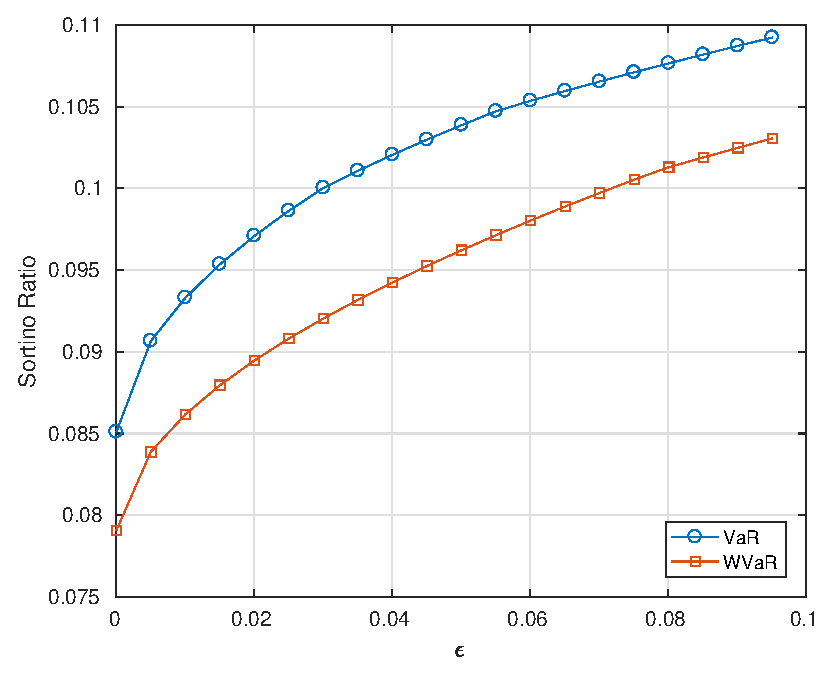
\includegraphics[height=7.0cm,width=0.7\textwidth]{VaR/bse30_market/sr_cheb.eps}
\caption{Sharpe ratio plot for Base VaR and WVaR models in case of Market data (31 assets)}
\label{fig:5.1}
\end{figure}

\begin{table}[!h]
\centering
\captionsetup{justification=centering}
\begin{tabular}{||c|c|c|c|c|c|c||}
\hline
$\epsilon$ & $\mu_{VaR}$ & $\sigma_{VaR}$ & $\mu_{WVaR}$ & $\sigma_{WVaR}$ & $SR_{VaR}$ & $SR_{WVaR}$\\
\hline
0.0001 & 0.000646 & 0.00522 & 0.000603 & 0.00528 & 0.0932 & 0.0839 \\
0.0201 & 0.000715 & 0.00522 & 0.00066 & 0.00529 & 0.106 & 0.0947 \\
0.0401 & 0.000744 & 0.00523 & 0.000687 & 0.0053 & 0.112 & 0.0995 \\
0.0601 & 0.000763 & 0.00523 & 0.000708 & 0.0053 & 0.115 & 0.103 \\
0.0801 & 0.000777 &0.00524 & 0.000726 & 0.00531 & 0.118 & 0.107 \\
\hline
& & & & Avg & 0.111	& 0.0998 \\
\hline
\end{tabular}
\caption{Empirical Analysis of Base VaR and WVaR models in case of Market Data (31 assets)}
\label{tab:5.1}
\end{table}

\begin{figure}[!h]
\centering
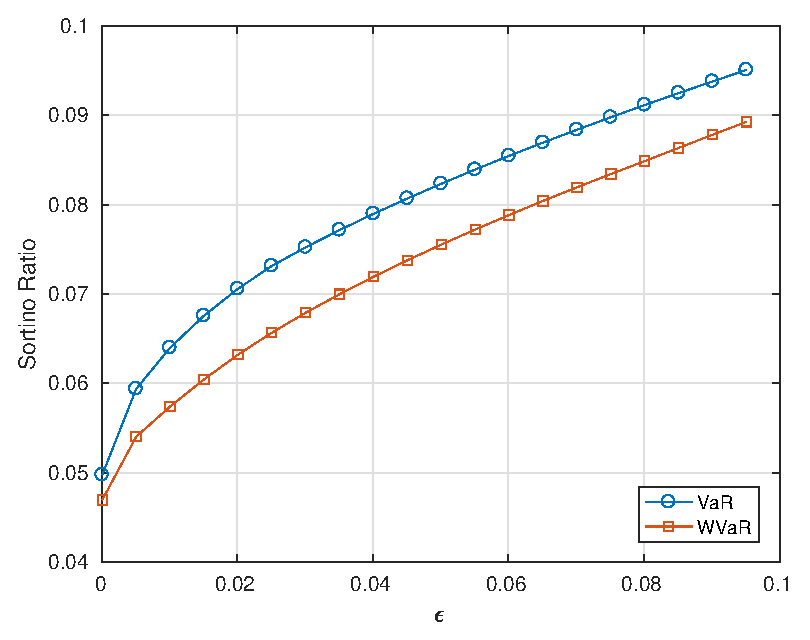
\includegraphics[height=7.0cm,width=0.7\textwidth]{VaR/bse30_simulated/sr_exact_cheb.eps}
\caption{Sharpe ratio plot for Base VaR and WVaR models in case of simulated data with $\zeta$ number of samples (31 assets)}
\label{fig:5.2}
\end{figure}


\begin{table}[!h]
\centering
\captionsetup{justification=centering}
\begin{tabular}{||c|c|c|c|c|c|c||}
\hline
$\epsilon$ & $\mu_{VaR}$ & $\sigma_{VaR}$ & $\mu_{WVaR}$ & $\sigma_{WVaR}$ & $SR_{VaR}$ & $SR_{WVaR}$\\
\hline
0.0001 & 0.000444 & 0.00509 & 0.000417 & 0.00519 & 0.0557 & 0.0496 \\
0.0201 & 0.000562 & 0.0051 & 0.000506 & 0.0052 & 0.0788 & 0.0665 \\
0.0401 & 0.00061 & 0.00511 & 0.000554 & 0.00521 & 0.0881 & 0.0756 \\
0.0601 & 0.000647 & 0.00512 & 0.000592 & 0.00522 & 0.0953 & 0.0828 \\
0.0801 & 0.000681 & 0.00513 & 0.000625 & 0.00523 & 0.102 & 0.089 \\
\hline
& & & & Avg & 0.0884 & 0.0765 \\
\hline
\end{tabular}
\caption{Empirical Analysis of Base VaR and WVaR models in case of simulated data with $\zeta$ number of samples (31 assets)}
\label{tab:5.2}
\end{table}

\begin{figure}[!h]
\centering
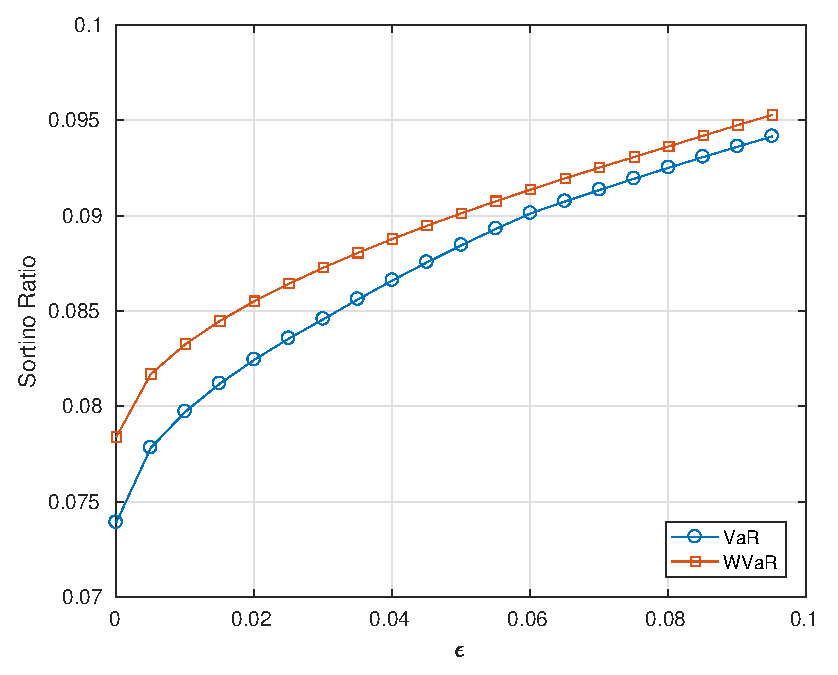
\includegraphics[height=7.0cm,width=0.7\textwidth]{VaR/bse30_simulated/sr_1000_cheb.eps}
\caption{Sharpe ratio plot for Base VaR and WVaR models in case of simulated data with 1000 samples (31 assets)}
\label{fig:5.3}
\end{figure}

\begin{table}[!h]
\centering
\captionsetup{justification=centering}
\begin{tabular}{||c|c|c|c|c|c|c||}
\hline
$\epsilon$ & $\mu_{VaR}$ & $\sigma_{VaR}$ & $\mu_{WVaR}$ & $\sigma_{WVaR}$ & $SR_{VaR}$ & $SR_{WVaR}$\\
\hline
0.0001 & 0.000587 & 0.00507 & 0.000605 & 0.0051 & 0.0842 & 0.0873 \\
0.0201 & 0.000636 & 0.00508 & 0.000645 & 0.0051 & 0.0937 & 0.0951 \\
0.0401 & 0.00066 & 0.00508 & 0.000663 & 0.00511 & 0.0984 & 0.0986 \\
0.0601 & 0.00068 & 0.00509 & 0.000678 & 0.00511 & 0.102 & 0.101 \\
0.0801 & 0.000694 & 0.00509 & 0.000691 & 0.00512 & 0.105 & 0.104 \\
\hline
& & & & Avg & 0.0987 & 0.0989 \\
\hline
\end{tabular}
\caption{Empirical Analysis of Base VaR and WVaR models in case of simulated data with 1000 samples (31 assets)}
\label{tab:5.3}
\end{table}

\begin{figure}[!h]
\centering
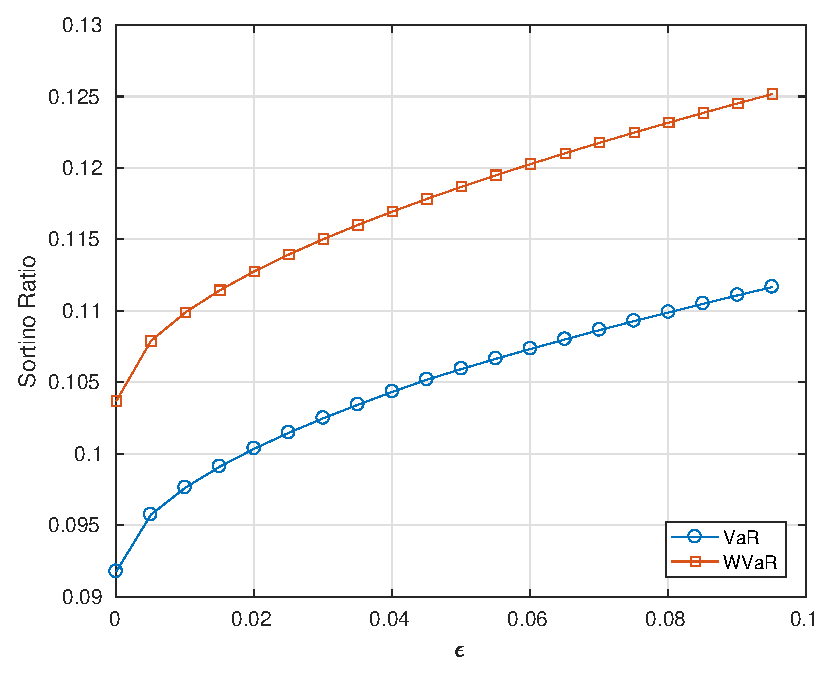
\includegraphics[height=7.0cm,width=0.7\textwidth]{VaR/bse100_market/sr_cheb.eps}
\caption{Sharpe ratio plot for Base VaR and WVaR models in case of market data (98 assets)}
\label{fig:5.4}
\end{figure}

\begin{table}[!h]
\centering
\captionsetup{justification=centering}
\begin{tabular}{||c|c|c|c|c|c|c||}
\hline
$\epsilon$ & $\mu_{VaR}$ & $\sigma_{VaR}$ & $\mu_{WVaR}$ & $\sigma_{WVaR}$ & $SR_{VaR}$ & $SR_{WVaR}$\\
\hline
0.0001 & 0.000667 & 0.00484 & 0.00071 & 0.00496 & 0.105 & 0.111 \\ 
0.0201 & 0.000713 & 0.00485 & 0.000755 & 0.00497 & 0.114 & 0.12 \\
0.0401 & 0.000735 & 0.00485 & 0.000776 & 0.00498 & 0.119 & 0.124 \\
0.0601 & 0.000751 & 0.00486 & 0.000793 & 0.00499 & 0.122 & 0.127 \\
0.0801 & 0.000765 & 0.00486 & 0.000807 & 0.005 & 0.124 & 0.13 \\
\hline
& & & & Avg & 0.119 & 0.124 \\
\hline
\end{tabular}
\caption{Empirical Analysis of Base VaR and WVaR models in case of market data (98 assets)}
\label{tab:5.4}
\end{table}

\begin{figure}[!h]
\centering
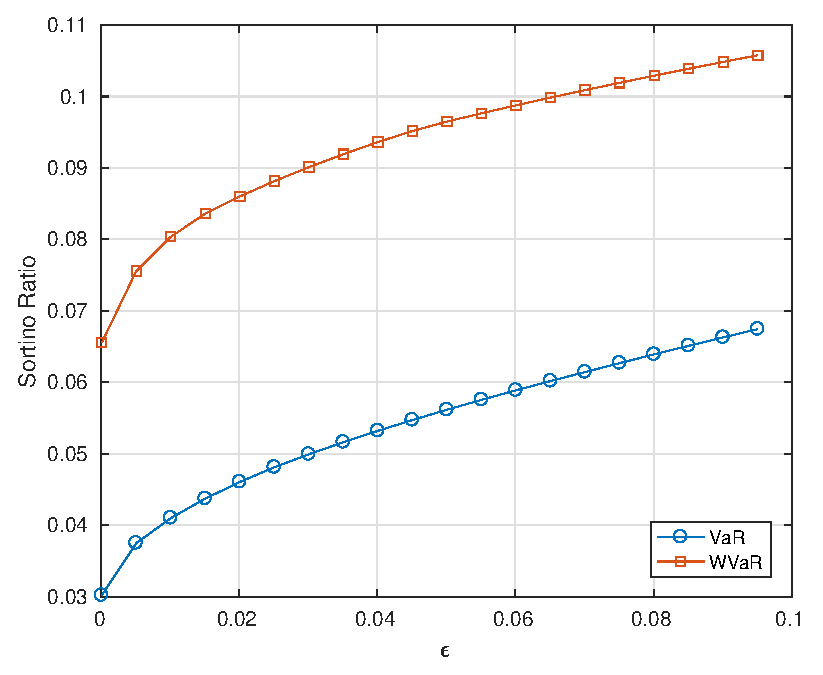
\includegraphics[height=7.0cm,width=0.7\textwidth]{VaR/bse100_simulated/sr_exact_cheb.eps}
\caption{Sharpe ratio plot for Base VaR and WVaR models in case of simulated data with $\zeta$ number of samples (98 assets)}
\label{fig:5.5}
\end{figure}

\begin{table}[!h]
\centering
\captionsetup{justification=centering}
\begin{tabular}{||c|c|c|c|c|c|c||}
\hline
$\epsilon$ & $\mu_{VaR}$ & $\sigma_{VaR}$ & $\mu_{WVaR}$ & $\sigma_{WVaR}$ & $SR_{VaR}$ & $SR_{WVaR}$\\
\hline
0.0001 & 0.000341 & 0.00471 & 0.00052 & 0.00487 & 0.0384 & 0.074 \\
0.0201 & 0.000434 & 0.00472 & 0.000629 & 0.00491 & 0.0581 & 0.0957 \\
0.0401 & 0.000475 & 0.00473 & 0.00067 & 0.00493 & 0.0668 & 0.104 \\
0.0601 & 0.000508 & 0.00473 & 0.000697 & 0.00494 & 0.0736 & 0.109 \\
0.0801 & 0.000537 & 0.00474 & 0.000719 & 0.00495 & 0.0796 & 0.113 \\ 
\hline
& & & & Avg & 0.0674 & 0.103 \\
\hline
\end{tabular}
\caption{Empirical Analysis of Base VaR and WVaR models in case of simulated data with $\zeta$ number of samples(98 assets)}
\label{tab:5.5}
\end{table}

\begin{figure}[!h]
\centering
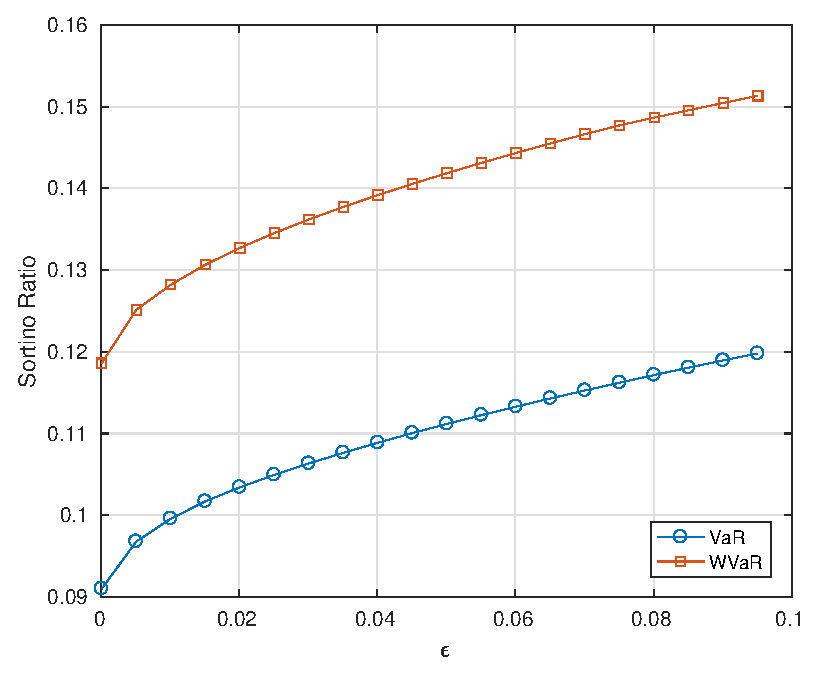
\includegraphics[height=7.0cm,width=0.7\textwidth]{VaR/bse100_simulated/sr_1000_cheb.eps}
\caption{Sharpe ratio plot for Base VaR and WVaR models in case of simulated data with 1000 samples (98 assets)}
\label{fig:5.6}
\end{figure}

\begin{table}[!h]
\centering
\captionsetup{justification=centering}
\begin{tabular}{||c|c|c|c|c|c|c||}
\hline
$\epsilon$ & $\mu_{VaR}$ & $\sigma_{VaR}$ & $\mu_{WVaR}$ & $\sigma_{WVaR}$ & $SR_{VaR}$ & $SR_{WVaR}$\\
\hline
0.0001 & 0.000702 & 0.00471 & 0.000822 & 0.0048 & 0.115 & 0.138 \\
0.0201 & 0.000772 & 0.00472 & 0.000897 & 0.00483 & 0.13 & 0.153 \\
0.0401 & 0.000803 & 0.00472 & 0.000931 & 0.00484 & 0.136 & 0.16 \\
0.0601 & 0.000828 & 0.00473 & 0.000959 & 0.00485 & 0.141 & 0.165 \\
0.0801 & 0.00085 & 0.00474 & 0.000982 & 0.00486 & 0.146 & 0.169 \\
\hline
& & & & Avg & 0.137 & 0.16 \\
\hline
\end{tabular}
\caption{Empirical Analysis of Base VaR and WVaR models in case of simulated data with 1000 samples (98 assets)}
\label{tab:5.6}
\end{table}

\begin{table}[!h]
    \centering
    \captionsetup{justification=centering}

   \begin{tabular}{||c|c|c|c||}
   \hline
  
$l$ & $Avg. \, \, SR_{CVaR}$ & $Avg. \, \, SR_{WCVaR}$ & $Diff. \, \, in \, \, Avg. \, \, SR$ \\
  
  \hline
2 & 0.0856 & 0.0611 & -0.0245 \\
3 & 0.0856 & 0.0345 & -0.0511 \\
4 & 0.0856 & 0.0439 & -0.0417 \\
5 & 0.0856 & 0.031 & -0.0546 \\
  \hline
\end{tabular}
    \caption{Comparison of CVaR and WCVaR in case of Market Data (31 assets) for different values of $l$}
    \label{avgtab:6.1}
\end{table}

\begin{figure}[!h]
    \centering
   
    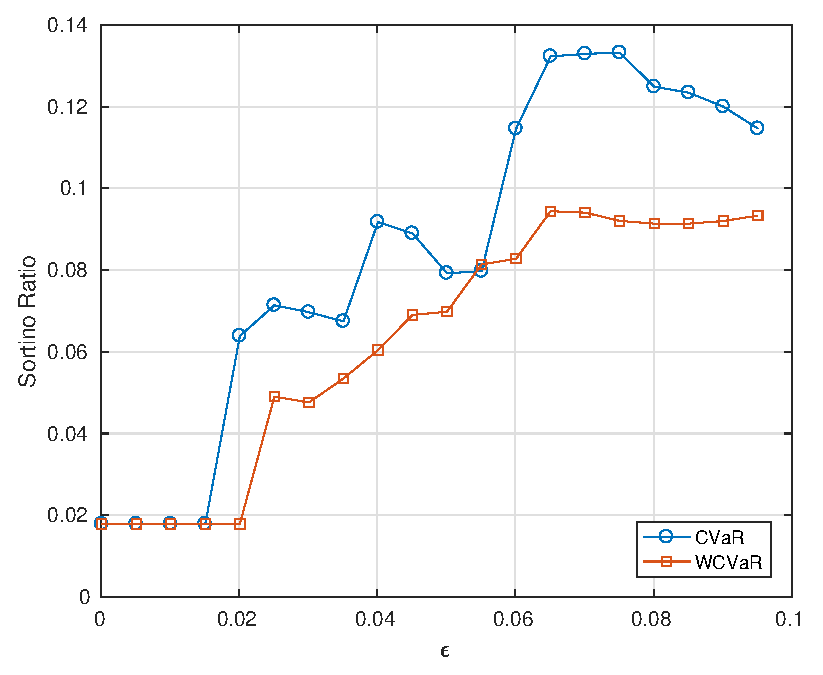
\includegraphics[height=7.0cm,width=0.7\textwidth]{CVaR/bse30_market/sr_cvar_2.eps}

   \caption{Sharpe ratio plot for CVaR and WCVaR in case of Market Data (31 assets) for $l=2$}
   \label{fig:6.1}
\end{figure}

\begin{table}[!h]
    \centering
    \captionsetup{justification=centering}

   \begin{tabular}{||c|c|c|c|c|c|c||}
   \hline
  
$\epsilon$ & $\mu_{CVaR}$ & $\sigma_{CVaR}$ & $\mu_{WCVaR}$ & $\sigma_{WCVaR}$ & $SR_{CVaR}$ & $SR_{WCVaR}$\\
  
  \hline
0.0001 & 0.000266 & 0.00661 & 0.000266 & 0.00661 & 0.0162 & 0.0162 \\
0.0201 & 0.000545 & 0.00595 & 0.000266 & 0.00661 & 0.0648 & 0.0162 \\
0.0401 & 0.000706 & 0.00569 & 0.000514 & 0.00603 & 0.096 & 0.0587 \\
0.0601 & 0.000832 & 0.00557 & 0.000645 & 0.00598 & 0.121 & 0.0812 \\
0.0801 & 0.000877 & 0.00576 & 0.000696 & 0.00597 & 0.125 & 0.0897 \\
  \hline
\end{tabular}
    \caption{Empirical Analysis of CVaR and WCVaR in case of Market Data (31 assets) for $l=2$}
    \label{tab:6.1}
\end{table}

\begin{table}[!h]
    \centering
    \captionsetup{justification=centering}

   \begin{tabular}{||c|c|c|c||}
   \hline
  
$l$ & $Avg. \, \, SR_{CVaR}$ & $Avg. \, \, SR_{WCVaR}$ & $Diff. \, \, in \, \, Avg. \, \, SR$ \\
  
  \hline
2 & 0.103 & 0.102 & -0.000411 \\
3 & 0.103 & 0.103 & 0.000195 \\
4 & 0.103 & 0.104 & 0.00124 \\
5 & 0.103 & 0.106 & 0.00358 \\
  \hline
\end{tabular}
    \caption{Comparison of CVaR and WCVaR in case of Simulated Data with $\zeta$ samples (31 assets) for different values of $l$}
    \label{avgtab:6.2}
\end{table}

\begin{figure}[!h]
    \centering
   
    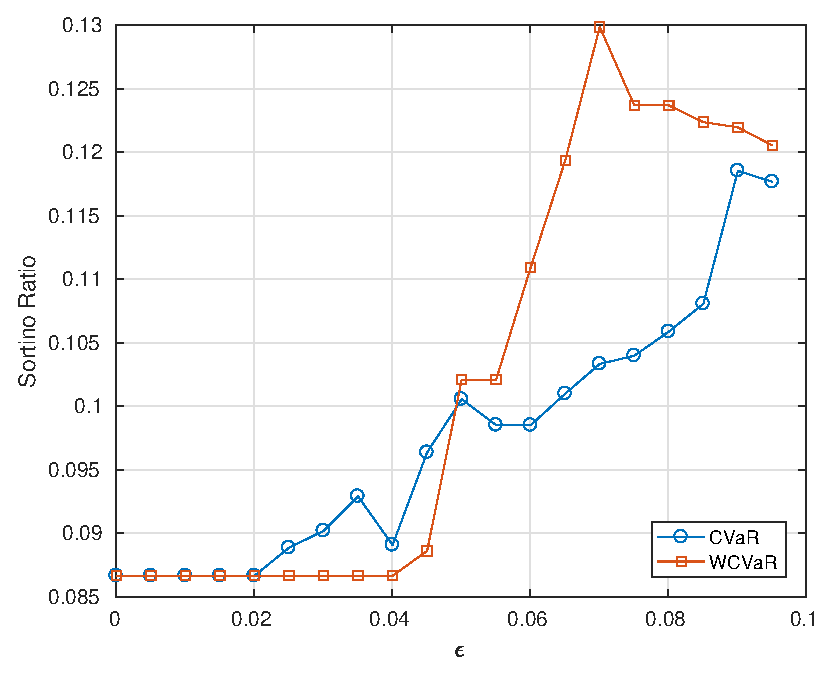
\includegraphics[height=7.0cm,width=0.7\textwidth]{CVaR/bse30_simulated/sr_exact_5.eps}

   \caption{Sharpe ratio plot for CVaR and WCVaR in case of Simulated Data with $\zeta$ samples (31 assets) for $l=5$}
   \label{fig:6.2}
\end{figure}

\begin{table}[!h]
    \centering
    \captionsetup{justification=centering}

   \begin{tabular}{||c|c|c|c|c|c|c||}
   \hline
  
$\epsilon$ & $\mu_{CVaR}$ & $\sigma_{CVaR}$ & $\mu_{WCVaR}$ & $\sigma_{WCVaR}$ & $SR_{CVaR}$ & $SR_{WCVaR}$\\
  
  \hline
0.0001 & 0.000675 & 0.00587 & 0.000675 & 0.00587 & 0.0878 & 0.0878 \\
0.0201 & 0.000675 & 0.00587 & 0.000675 & 0.00587 & 0.0878 & 0.0878 \\
0.0401 & 0.000694 & 0.00559 & 0.000675 & 0.00587 & 0.0957 & 0.0878 \\
0.0601 & 0.000731 & 0.00542 & 0.000838 & 0.00607 & 0.105 & 0.112 \\
0.0801 & 0.000776 & 0.00541 & 0.000889 & 0.00545 & 0.114 & 0.134 \\
  \hline
\end{tabular}
    \caption{Empirical Analysis of CVaR and WCVaR in case of Simulated Data with $\zeta$ samples (31 assets) for $l=5$}
    \label{tab:6.2}
\end{table}

\begin{table}[!h]
    \centering
    \captionsetup{justification=centering}

   \begin{tabular}{||c|c|c|c||}
   \hline
  
$l$ & $Avg. \, \, SR_{CVaR}$ & $Avg. \, \, SR_{WCVaR}$ & $Diff. \, \, in \, \, Avg. \, \, SR$ \\
  
  \hline
2 & 0.0929 & 0.0967 & 0.00374 \\
3 & 0.0929 & 0.0945 & 0.00161 \\
4 & 0.0929 & 0.0969 & 0.00402 \\
5 & 0.0929 & 0.0954 & 0.00249 \\
  \hline
\end{tabular}
    \caption{Comparison of CVaR and WCVaR in case of Simulated Data with $1000$ samples (31 assets) for different values of $l$}
    \label{avgtab:6.3}
\end{table}

\begin{figure}[!h]
    \centering
   
    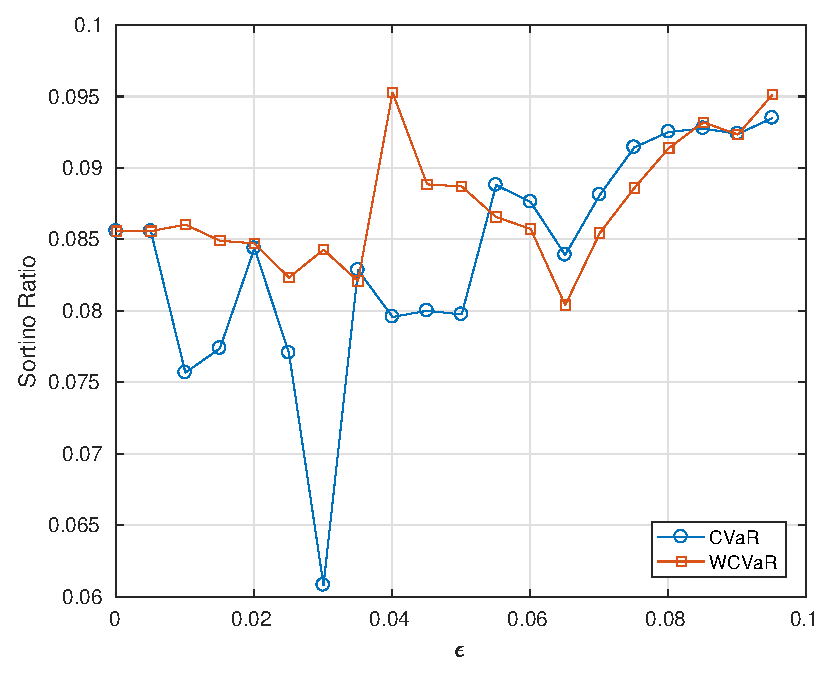
\includegraphics[height=7.0cm,width=0.7\textwidth]{CVaR/bse30_simulated/sr_1000_4.eps}

   \caption{Sharpe ratio plot for CVaR and WCVaR in case of Simulated Data with $1000$ samples (31 assets) for $l=4$}
   \label{fig:6.3}
\end{figure}

\begin{table}[!h]
    \centering
    \captionsetup{justification=centering}

   \begin{tabular}{||c|c|c|c|c|c|c||}
   \hline
  
$\epsilon$ & $\mu_{CVaR}$ & $\sigma_{CVaR}$ & $\mu_{WCVaR}$ & $\sigma_{WCVaR}$ & $SR_{CVaR}$ & $SR_{WCVaR}$\\
  
  \hline
0.0001 & 0.000677 & 0.00563 & 0.000677 & 0.00563 & 0.0919 & 0.0919 \\
0.0201 & 0.000658 & 0.0054 & 0.000661 & 0.0054 & 0.0923 & 0.0929 \\
0.0401 & 0.000629 & 0.00534 & 0.000722 & 0.00531 & 0.0879 & 0.106 \\
0.0601 & 0.00067 & 0.00523 & 0.000667 & 0.00526 & 0.0976 & 0.0965 \\
0.0801 & 0.000701 & 0.0052 & 0.000692 & 0.00519 & 0.104 & 0.103 \\
  \hline
\end{tabular}
    \caption{Empirical Analysis of CVaR and WCVaR in case of Simulated Data with $1000$ samples (31 assets) for $l=4$}
    \label{tab:6.3}
\end{table}

\begin{table}[!h]
    \centering
    \captionsetup{justification=centering}

   \begin{tabular}{||c|c|c|c||}
   \hline
  
$l$ & $Avg. \, \, SR_{CVaR}$ & $Avg. \, \, SR_{WCVaR}$ & $Diff. \, \, in \, \, Avg. \, \, SR$ \\
  
  \hline
2 & 0.121 & 0.102 & -0.0189 \\
3 & 0.121 & 0.105 & -0.0165 \\
4 & 0.121 & 0.0991 & -0.0219 \\
5 & 0.121 & 0.0927 & -0.0283 \\
  \hline
\end{tabular}
    \caption{Comparison of CVaR and WCVaR in case of Market Data (98 assets) for different values of $l$}
    \label{avgtab:6.4}
\end{table}

\begin{figure}[!h]
    \centering
   
    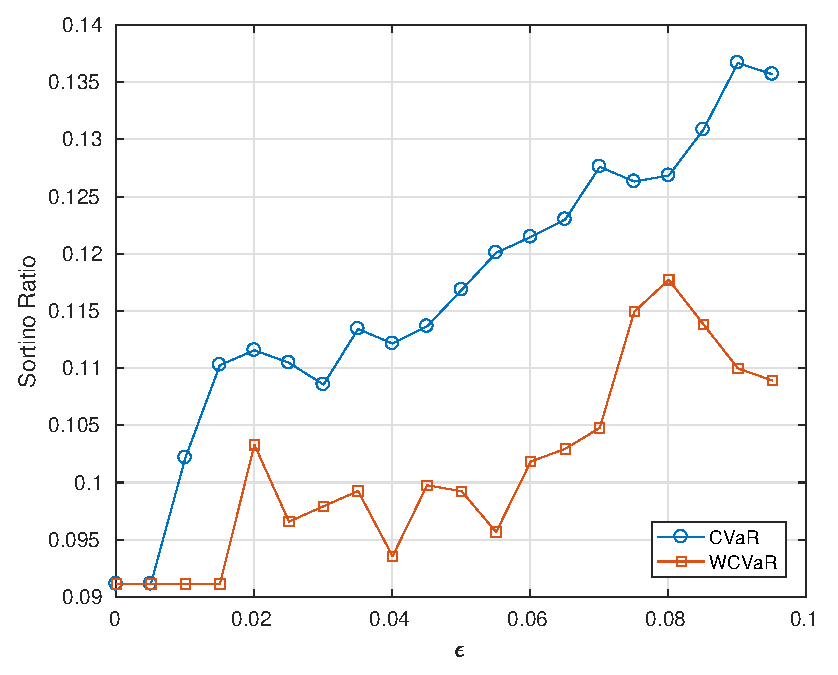
\includegraphics[height=7.0cm,width=0.7\textwidth]{CVaR/bse100_market/sr_cvar_3.eps}

   \caption{Sharpe ratio plot for CVaR and WCVaR in case of Market Data (98 assets) for $l=3$}
   \label{fig:6.4}
\end{figure}

\begin{table}[!h]
    \centering
    \captionsetup{justification=centering}

   \begin{tabular}{||c|c|c|c|c|c|c||}
   \hline
  
$\epsilon$ & $\mu_{CVaR}$ & $\sigma_{CVaR}$ & $\mu_{WCVaR}$ & $\sigma_{WCVaR}$ & $SR_{CVaR}$ & $SR_{WCVaR}$\\
  
  \hline
0.0001 & 0.000687 & 0.00593 & 0.000687 & 0.00593 & 0.0889 & 0.0889 \\
0.0201 & 0.000786 & 0.00544 & 0.000755 & 0.00582 & 0.115 & 0.102 \\
0.0401 & 0.00079 & 0.00535 & 0.000692 & 0.0055 & 0.118 & 0.0967 \\
0.0601 & 0.000839 & 0.00537 & 0.000738 & 0.00533 & 0.127 & 0.108 \\
0.0801 & 0.000847 & 0.00517 & 0.00082 & 0.00531 & 0.133 & 0.124 \\
  \hline
\end{tabular}
    \caption{Empirical Analysis of CVaR and WCVaR in case of Market Data (98 assets) for $l=3$}
    \label{tab:6.4}
\end{table}

\begin{table}[!h]
    \centering
    \captionsetup{justification=centering}

   \begin{tabular}{||c|c|c|c||}
   \hline
  
$l$ & $Avg. \, \, SR_{CVaR}$ & $Avg. \, \, SR_{WCVaR}$ & $Diff. \, \, in \, \, Avg. \, \, SR$ \\
  
  \hline
2 & 0.0963 & 0.0978 & 0.00156 \\
3 & 0.0963 & 0.0968 & 0.000541 \\
4 & 0.0963 & 0.102 & 0.00581 \\
5 & 0.0963 & 0.0915 & -0.00479 \\
  \hline
\end{tabular}
    \caption{Comparison of CVaR and WCVaR in case of Simulated Data with $\zeta$ samples (98 assets) for different values of $l$}
    \label{avgtab:6.5}
\end{table}

\begin{figure}[!h]
    \centering
   
    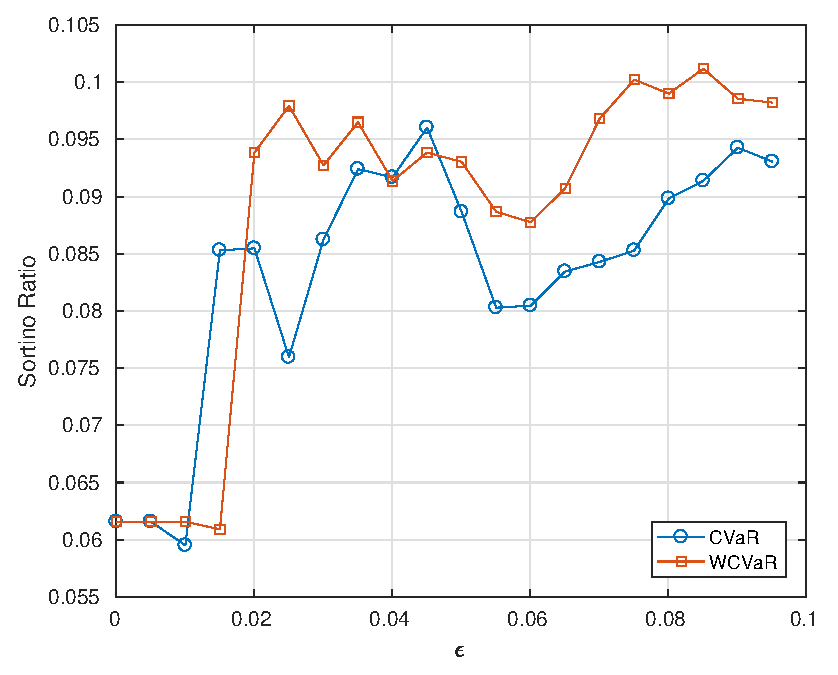
\includegraphics[height=7.0cm,width=0.7\textwidth]{CVaR/bse100_simulated/sr_exact_4.eps}

   \caption{Sharpe ratio plot for CVaR and WCVaR in case of Simulated Data with $\zeta$ samples (98 assets) for $l=4$}
   \label{fig:6.5}
\end{figure}

\begin{table}[!h]
    \centering
    \captionsetup{justification=centering}

   \begin{tabular}{||c|c|c|c|c|c|c||}
   \hline
  
$\epsilon$ & $\mu_{CVaR}$ & $\sigma_{CVaR}$ & $\mu_{WCVaR}$ & $\sigma_{WCVaR}$ & $SR_{CVaR}$ & $SR_{WCVaR}$\\
  
  \hline
0.0001 & 0.000554 & 0.00579 & 0.000554 & 0.00579 & 0.0681 & 0.0681 \\
0.0201 & 0.000703 & 0.0055 & 0.000755 & 0.00547 & 0.0988 & 0.109 \\
0.0401 & 0.000727 & 0.00546 & 0.000723 & 0.00536 & 0.104 & 0.105 \\
0.0601 & 0.000648 & 0.00522 & 0.000698 & 0.00527 & 0.0935 & 0.102 \\
0.0801 & 0.000706 & 0.00514 & 0.000768 & 0.00525 & 0.106 & 0.116 \\
  \hline
\end{tabular}
    \caption{Empirical Analysis of CVaR and WCVaR in case of Simulated Data with $\zeta$ samples (98 assets) for $l=4$}
    \label{tab:6.5}
\end{table}

\begin{table}[!h]
    \centering
    \captionsetup{justification=centering}

   \begin{tabular}{||c|c|c|c||}
   \hline
  
$l$ & $Avg. \, \, SR_{CVaR}$ & $Avg. \, \, SR_{WCVaR}$ & $Diff. \, \, in \, \, Avg. \, \, SR$ \\
  
  \hline
2 & 0.156 & 0.156 & -0.000382 \\
3 & 0.156 & 0.16 & 0.0037 \\
4 & 0.156 & 0.163 & 0.00667 \\
5 & 0.156 & 0.165 & 0.00868 \\
  \hline
\end{tabular}
    \caption{Comparison of CVaR and WCVaR in case of Simulated Data with $1000$ samples (98 assets) for different values of $l$}
    \label{avgtab:6.6}
\end{table}

\begin{figure}[!h]
    \centering
   
    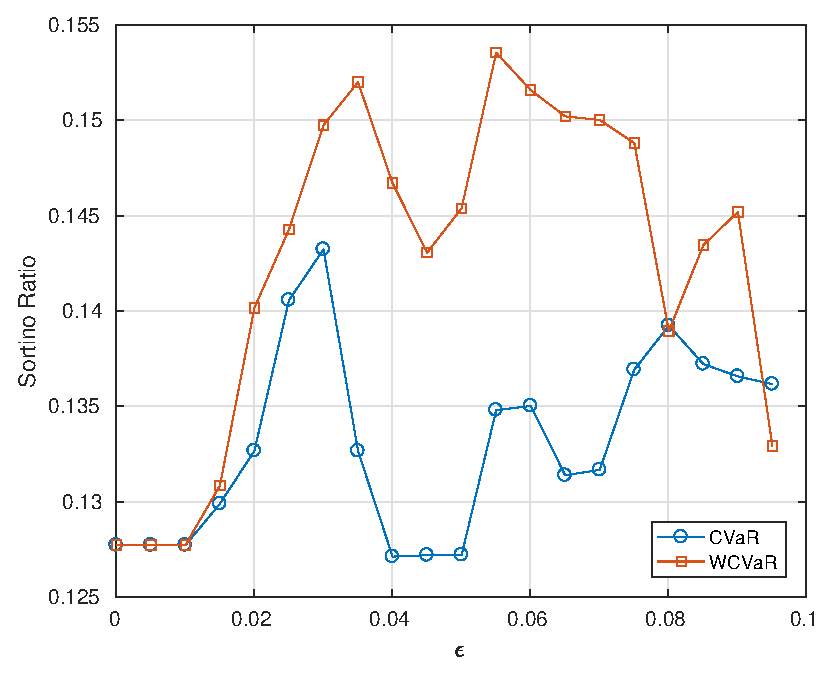
\includegraphics[height=7.0cm,width=0.7\textwidth]{CVaR/bse100_simulated/sr_1000_5.eps}

   \caption{Sharpe ratio plot for CVaR and WCVaR in case of Simulated Data with $1000$ samples (98 assets) for $l=5$}
   \label{fig:6.6}
\end{figure}

\begin{table}[!h]
    \centering
    \captionsetup{justification=centering}

   \begin{tabular}{||c|c|c|c|c|c|c||}
   \hline
  
$\epsilon$ & $\mu_{CVaR}$ & $\sigma_{CVaR}$ & $\mu_{WCVaR}$ & $\sigma_{WCVaR}$ & $SR_{CVaR}$ & $SR_{WCVaR}$\\
  
  \hline
0.0001 & 0.000935 & 0.00536 & 0.000935 & 0.00536 & 0.145 & 0.145 \\
0.0201 & 0.00097 & 0.00537 & 0.00101 & 0.00536 & 0.151 & 0.159 \\
0.0401 & 0.000927 & 0.0051 & 0.00104 & 0.00531 & 0.15 & 0.166 \\
0.0601 & 0.000963 & 0.00496 & 0.00106 & 0.00504 & 0.162 & 0.179 \\
0.0801 & 0.000974 & 0.00489 & 0.000981 & 0.00495 & 0.167 & 0.166 \\
  \hline
\end{tabular}
    \caption{Empirical Analysis of CVaR and WCVaR in case of Simulated Data with $1000$ samples (98 assets) for $l=5$}
    \label{tab:6.6}
\end{table}


\end{document}